\section{Theory}
\subsection{The data set}
As mentioned in the introduction The data set chosen is payment data 
from an important bank in Taiwan, where the data describes credit card holders,
and the goal is predicting whether a customer will default the next 
payment or not.

The data is from 2005. Among the total 25,000 observations, 5529 observations
(22.12\%) are the cardholders with default payment.~\cite{ComparisonData} 

The research of this data set  employed a binary variable, default payment 
(Yes = 1, No = 0), as the response variable. The study reviewed the 
literature and used the following 23 variables as explanatory variables: 
\begin{itemize}
		\item
X1: Amount of the given credit (NT dollar): it includes both the individual consumer credit and his/her family (supplementary) credit. 
\item
X2: Gender (1 = male; 2 = female). 
\item
X3: Education (1 = graduate school; 2 = university; 3 = high school; 4 = others). 
\item
X4: Marital status (1 = married; 2 = single; 3 = others). 
\item
X5: Age (year).
\item
X6 - X11: History of past payment. We tracked the past monthly payment records (from April to September, 2005) as follows: X6 = the repayment status in September, 2005; X7 = the repayment status in August, 2005; . . .;X11 = the repayment status in April, 2005. The measurement scale for the repayment status is: -1 = pay duly; 1 = payment delay for one month; 2 = payment delay for two months; . . .; 8 = payment delay for eight months; 9 = payment delay for nine months and above. 
\item
X12-X17: Amount of bill statement (NT dollar). X12 = amount of bill statement in September, 2005; X13 = amount of bill statement in August, 2005; . . .; X17 = amount of bill statement in April, 2005. 
\item
X18-X23: Amount of previous payment (NT dollar). X18 = amount paid in September, 2005; X19 = amount paid in August, 2005; . . .;X23 = amount paid in April, 2005. 
\end{itemize} ~\cite{CreditCardData} 



The aim of doing a risk prediction is to reduce damage and 
uncertainty that occur when a bank over-issue cash and credit 
cards to unqualified cardholderst ~\cite{ComparisonData}

When such a crisis occur it is a challenge for both banks and 
cardholders, and a risk prediction is therefore a very useful tool. 


\subsection{Imbalanced Data in Classification}
A common challenge in classification is imbalanced data, in which a large
amount of the labeled data belongs to just one or a few of the classes.
For binary classification, if 90\% of the data belongs to one of the classes,
then the classifier is likely to end up placing every single
input in that class, as it will bring its accuracy to 90\%. Techincally, this
accuracy is correct, but it's not very useful since the decision isn't at all
affected by the features of the input. Accuracy alone isn't a good enough
measure of performance to reveal this.

Fortunately, since this is common, a number of methods have been developed
to combat the issue, some of which are described below.

\subsection{Resampling and Weighting}
In resampling there are essentially two main categories: Under-sampling
over-sampling. The difference between them is that over-sampling works with
somehow generating more samples of the minority class, while under-sampling
uses a reduced amount of samples from the majority class.
Weighting the samples is a differente approach in which the samples labeled
as the minority class are weighted higher than the others during training.

\subsubsection{Naive Random Over-sampling}
A very straightforward way to balance a dataset, is to choose random samples 
from the minority class, with replacement, until there is roughly equal
amounts of samples belonging to each class.

\subsubsection{SMOTE}
SMOTE - Synthetic Minority Over-sampling Technique, as the name suggests will
actually synthesize samples from the minority class in order to over-sample,
instead of sampling with replacement. This is done by taking each minority 
class sample and introducing synthetic examples along the line segments joining 
any/all of the k minority class nearest neighbors. Depending upon the amount of 
over-sampling required, neighbors from the k nearest neighbors are randomly
chosen. The result of synthesizing rather than choosing with replacement is
that the decision region is forced to become more general.
See \cite{smote-article} for a more detailed explanation of the methods
involved.

\subsubsection{ADASYN}
Like SMOTE, ADASYN (Adaptive Synthetic Sampling) generates synthetic samples
in order to balance the number of samples in each class. The difference is
mainly that ADASYN uses a density distribution as a criterion to automatically 
decide the number of synthetic samples for each sample in the minority class.
The density distribution is a measurement of the distribution of weight for 
different minority class examples according to their level of difficulty in
learning. This way, ADASYN effectively forces the learning algorithm to 
focus more on examples that are difficult to learn.

\subsubsection{Balanced Weighting}
Scikit-learn's logistic regressor comes with it's own form of handling of
imbalanced data - weighting. It is a streightforward approach in which 
the values of targets are used to to automatically adjust weights inversely 
proportional to class frequencies in the input data as 
$$\frac{samples}{classes \cdot np.bincount(targets)}$$

\subsection{Assessing the Performance of Models}
If classification accuracy is not enough to gauge whether a model is
performing well, or well in the desired way, alternative way to measure
performance must be explored. For cases of imbalanced data there are a few
widely used methods that reveal information about the model that the simple
accuracy metric can't.

\subsubsection{Confusion Matrix}
A confusion matrix is an n by n matrix containing correct classifications
on the diagonal, and false positives and negatives in the off-diagonal elements.
An example of such a matrix could be the following table:
\begin{table}[h]
    \centering
    \begin{tabular}{c|c|c|c}
     & True Cat & True Dog & True Rabbit \\
    \hline
    Predicted Cat & \textbf{5} & 2 & 0 \\
    \hline
    Predicted Dog & 3 & \textbf{3} & 2 \\
    \hline
    Predicted Rabbit & 0 & 1 & \textbf{11} \\
\end{tabular}
\caption{Confusion matrix for an example classification where the classes
         are Cat, Dog and Rabbit. Correct classifications in bold.}
\label{tab:confmat-example}
\end{table}
In the table above (\ref{tab:confmat-example}), the diagonal elements
$i = j$ are the correct classifications, while the other elements correspond
to cases where the model predicted class $i$ but should've predicted class $j$.
The confusion matrix thus gives information about false positives and false 
negatives, in addition to classification accuracy. This is very useful
in cases where for example false positives can be readily ignored or filtere
later, but false negatives may have severe consequences. An example of this
could be detection of cancer, in which a false positive can be ruled out
from further testing, while a false negative may lead to a patient being sent
home when actually needing help. For a more in-depth look at confusion matrices
see \cite{roc-article}.
\subsubsection{Cumulative Gains Chart}
Cumulative Gains Charts, often referred to as 'Lift Charts' (actually different
ways to represent the same concept), can be used to gain a different insight.
The chart lets us compare a binary classifier to both an ideal case and a
'random choice' case at the same time. The ideal classifier will predict an
input's category with 100\% confidence, so the probability will be 1.0 for
the correct class and 0 for the wrong class. Sorting the predicted
probabilities for the desired class (usually class 1) in descending order,
will for the ideal case leave all members for class 1 on top, and plotting
them in the order of appearance will give a steep curve. Random choice is
used as a baseline for the chart, and plotting the model's curve should
place it in between the random choice and ideal case. An example is shown in
figure \ref{fig:cumul-example}.
\begin{figure}[h]
    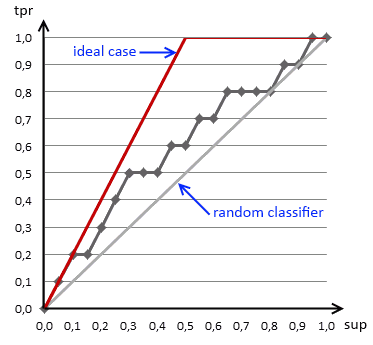
\includegraphics[width=0.7\textwidth]{figures/gain-chart}
    \caption{Example of a cumulative gain chart. Image borrowed from
    \cite{gains-example-image}.}
    \label{fig:cumul-example}
\end{figure}

\subsubsection{Receiver Operating Characteristic}
The Receiver Operating Characteristic (ROC) is a widely used measure of a 
classifiers performance . The performance is measured as the effect
of the true positive rate (TPR) and the false positive rate (FPR) as a function 
of thresholding the positive class. To evaluate the ROC curve for a model, 
traditionally the Area Under the Curve (AUC) is used, which ranges from 0 
(an ideal "opposite" classifier) to 1.0 (an ideal classifier) with 0.5 
indicating a random choice classifier, \cite{bertbert-article}(III.c).
For a thorough explanation of ROC curves and the underlying concepts, see \cite{roc-article}.

